\documentclass[a4paper]{article}

%plastikovye pakety

\usepackage[12pt]{extsizes}
\usepackage[utf8]{inputenc}
\usepackage[unicode, pdftex]{hyperref}
\usepackage{cmap}
\usepackage{mathtext}
\usepackage{multicol}
\setlength{\columnsep}{1cm}
\usepackage[T2A]{fontenc}
\usepackage[english,russian]{babel}
\usepackage{amsmath,amsfonts,amssymb,amsthm,mathtools}
\usepackage{icomma}
\usepackage{euscript}
\usepackage{mathrsfs}
\usepackage[dvipsnames]{xcolor}
\usepackage[left=2cm,right=2cm,
    top=2cm,bottom=2cm,bindingoffset=0cm]{geometry}
\usepackage[normalem]{ulem}
\usepackage{graphicx}
\usepackage{makeidx}
\usepackage{bbold}
\makeindex
\graphicspath{{pictures/}}
\DeclareGraphicsExtensions{.pdf,.png,.jpg}
%\usepackage[usenames]{color}
\hypersetup{
     colorlinks=true,
     linkcolor=brightturquoise,
     filecolor=brightturquoise,
     citecolor=black,      
     urlcolor=brightturquoise,
     }
\usepackage{fancyhdr}
\pagestyle{fancy} 
\fancyhead{} 
\fancyhead[LE,RO]{\thepage} 
\fancyhead[CO]{\hyperlink{uk}{к списку объектов}}
\fancyhead[LO]{\hyperlink{sod}{к содержанию}} 
\fancyfoot{}
\newtheoremstyle{indented}{0 pt}{0 pt}{\itshape}{}{\bfseries}{. }{0 em}{ }

\renewcommand\thesection{}
\renewcommand\thesubsection{}

%\geometry{verbose,a4paper,tmargin=2cm,bmargin=2cm,lmargin=2.5cm,rmargin=1.5cm}

\title{Теория категорий}
\author{Тутанов Михаил и Копейкина Софья\\ на основе лекций Петрова В.А.
\\ под редакцией @keba4ok}
\date{\today}


%envirnoments
    \theoremstyle{indented}
    \newtheorem{theorem}{Теорема}
    \newtheorem{lemma}{Лемма}
    \newtheorem{alg}{Алгоритм}

    \theoremstyle{definition} 
    \newtheorem{defn}{Определение}
    \newtheorem{exl}{Пример(ы)}
    \newtheorem{prob}{Задача}

    \theoremstyle{remark} 
    \newtheorem{remark}{Примечание}
    \newtheorem{cons}{Следствие}
    \newtheorem{exer}{Упражнение}
    \newtheorem{stat}{Утверждение}
%esli ne hochetsa numeracii - nuzhno prisunut' zvezdochku-pezsochku

\definecolor{brightturquoise}{rgb}{0.28, 0.82, 0.8}

%declarations
        %arrows_shorten
            \DeclareMathOperator{\la}{\leftarrow}
            \DeclareMathOperator{\ra}{\rightarrow}
            \DeclareMathOperator{\lra}{\leftrightarrow}
            \DeclareMathOperator{\llra}{\longleftrightarrow}
            \DeclareMathOperator{\La}{\Leftarrow}
            \DeclareMathOperator{\Ra}{\Rightarrow}
            \DeclareMathOperator{\Lra}{\Leftrightarrow}
            \DeclareMathOperator{\Llra}{\Longleftrightarrow}

        %letters_different
            \DeclareMathOperator{\CC}{\mathbb{C}}
            \DeclareMathOperator{\ZZ}{\mathbb{Z}}
            \DeclareMathOperator{\RR}{\mathbb{R}}
            \DeclareMathOperator{\NN}{\mathbb{N}}
            \DeclareMathOperator{\HH}{\mathbb{H}}
            \DeclareMathOperator{\LL}{\mathscr{L}}
            \DeclareMathOperator{\KK}{\mathscr{K}}
            \DeclareMathOperator{\GA}{\mathfrak{A}}
            \DeclareMathOperator{\GB}{\mathfrak{B}}
            \DeclareMathOperator{\GC}{\mathfrak{C}}
            \DeclareMathOperator{\GD}{\mathfrak{D}}
            \DeclareMathOperator{\GN}{\mathfrak{N}}
            \DeclareMathOperator{\Rho}{\mathcal{P}}
            \DeclareMathOperator{\FF}{\mathcal{F}}

        %common_shit
            \DeclareMathOperator{\Ker}{Ker}
            \DeclareMathOperator{\Frac}{Frac}
            \DeclareMathOperator{\Imf}{Im}
            \DeclareMathOperator{\cont}{cont}
            \DeclareMathOperator{\id}{id}
            \DeclareMathOperator{\ev}{ev}
            \DeclareMathOperator{\lcm}{lcm}
            \DeclareMathOperator{\chard}{char}
            \DeclareMathOperator{\codim}{codim}
            \DeclareMathOperator{\rank}{rank}
            \DeclareMathOperator{\ord}{ord}
            \DeclareMathOperator{\End}{End}
            \DeclareMathOperator{\Ann}{Ann}
            \DeclareMathOperator{\Real}{Re}
            \DeclareMathOperator{\Res}{Res}
            \DeclareMathOperator{\Rad}{Rad}
            \DeclareMathOperator{\disc}{disc}
            \DeclareMathOperator{\rk}{rk}
            \DeclareMathOperator{\const}{const}
            \DeclareMathOperator{\grad}{grad}
            \DeclareMathOperator{\Aff}{Aff}
            \DeclareMathOperator{\Lin}{Lin}
            \DeclareMathOperator{\Prf}{Pr}
            \DeclareMathOperator{\Iso}{Iso}
            \DeclareMathOperator{\Ob}{Ob}
            \DeclareMathOperator{\Hom}{Hom}

        %specific_shit
            \DeclareMathOperator{\Tors}{Tors}
            \DeclareMathOperator{\form}{Form}
            \DeclareMathOperator{\Pred}{Pred}
            \DeclareMathOperator{\Func}{Func}
            \DeclareMathOperator{\Const}{Const}
            \DeclareMathOperator{\arity}{arity}
            \DeclareMathOperator{\Aut}{Aut}
            \DeclareMathOperator{\Var}{Var}
            \DeclareMathOperator{\Term}{Term}
            \DeclareMathOperator{\sub}{sub}
            \DeclareMathOperator{\Sub}{Sub}
            \DeclareMathOperator{\Atom}{Atom}
            \DeclareMathOperator{\FV}{FV}
            \DeclareMathOperator{\Sent}{Sent}
            \DeclareMathOperator{\Th}{Th}
            \DeclareMathOperator{\supp}{supp}
            \DeclareMathOperator{\Eq}{Eq}
            \DeclareMathOperator{\Prop}{Prop}


%env_shortens_from_hirsh            
    \newcommand{\bex}{\begin{example}\rm}
    \newcommand{\eex}{\end{example}}
    \newcommand{\ba}{\begin{algorithm}\rm}
    \newcommand{\ea}{\end{algorithm}}
    \newcommand{\bea}{\begin{eqnarray*}}
    \newcommand{\eea}{\end{eqnarray*}}
    \newcommand{\be}{\begin{eqnarray}}
    \newcommand{\ee}{\end{eqnarray}}
    \newcommand{\abs}[1]{\lvert#1\rvert}
        \newcommand{\bp}{\begin{pr\Ob}}
        \newcommand{\ep}{\end{pr\Ob}}
    
\begin{document}
%ya_ebanutyi
\newcommand{\resetexlcounters}{%
  \setcounter{exl}{0}%
} 
\newcommand{\resetremarkcounters}{%
  \setcounter{remark}{0}%
} 
\newcommand{\reseconscounters}{%
  \setcounter{cons}{0}%
} 
\newcommand{\resetall}{%
    \resetexlcounters
    \resetremarkcounters
    \reseconscounters%
}
\newcommand{\cursed}[1]{\textit{\textcolor{brightturquoise}{#1}}}
\newcommand{\de}[3][2]{\index{#2}{\textbf{\textcolor{brightturquoise}{#3}}}}
\newcommand{\re}[3][2]{\hypertarget{#2}{\textbf{\textcolor{brightturquoise}{#3}}}}
\newcommand{\se}[3][2]{\index{#2}{\textit{\textcolor{brightturquoise}{#3}}}}
\maketitle 
\newpage
\hypertarget{sod}
\tableofcontents
\newpage
\section{Основные определения}
\begin{defn} 
\se{Категория}{Категория $\mathcal{C}$} -- это 
    \begin{itemize}
        \item класс\footnote{Если вдруг даже множество, то такая категория называется \textit{малой}} $\Ob\mathcal{C}$, элементы которого называются \textit{объектами};
        \item попарно непересекающиеся множества \textit{морфизмов} $\Hom (X, Y)$\footnote{Обозначение $Mor$ на мой взгляд логичнее, но используется сильно реже} для любых двух $X$ и $Y$ из $\Ob\mathcal{C}$;
        \item операция композиции $\circ $: $\Hom (Y, Z)\times \Hom (X, Y) \rightarrow \Hom (X, Z)$, удовлетворяющая двум аксиомам.
    \end{itemize}
\end{defn}
Аксиомы композиции: 
\begin{itemize}
    \item ассоциативность $(f\circ g)\circ h = f\circ (g\circ h)$;
    \item для любого $A$ из $\mathcal{C}$\footnote{$\Ob$ по-хорошему писать надо, но оно часто опускается} существует $\id_{A}\in{\Hom (A, A)}$ такое, что $f\circ \id_{A} = f$, $\id_{A}\circ f = f$ для любого осмысленного $f$.
\end{itemize}
\begin{defn}
    Два объекта $X$ и $Y$ в категории $\mathcal{C}$ называются \se{Изоморфные объекты}{изоморфными}, если $\exists f\in{\Hom (X, Y)}$ и $g\in{\Hom (Y, X)}$ такие, что $f\circ g=\id_{Y}$, $g\circ f=\id_{X}$. $f$ и $g$ в этом случае называются $\textit{изоморфизмами}$.
\end{defn}
\begin{defn}
    Объект $A$ в категории $\mathcal{C}$ называется \se{Терминальный объект}{терминальным} (\cursed{инициальным}), если для любого $X$ из $\mathcal{C}$ $\vert \Hom (X, A)\vert=1$ ($\vert \Hom (A, X)\vert=1$)
\end{defn}
\begin{stat}
    Если терминальный (инициальный) объект существует, то он единственен с точностью до единственного изоморфизма.
\end{stat}
\begin{proof}
    Пусть $A$ и $A'$ -- терминальные объекты, тогда из определения существует единственный $f$ из $A$ в $A'$ и единственный $g$ из $A'$ в $A$, композиция $f\circ g$ в этом случае будет элементом $\Hom (A', A')$, но $\id_{A'}$ также элемент этого одноэлементного множества, поэтому $f\circ g = \id_{A'}$, аналогично $g\circ f = \id_{A}$, то есть $A$ и $A'$ изоморфны по определению.
\end{proof}
Как можно заметить, инициальный и терминальный объекты подозрительно похожи, для того, чтобы формализовать наше подозрение, введём понятие двойственной (противоположной) категории.
\begin{defn}
    Для категории $\mathcal{C}$ определим следующую категорию $\mathcal{C}^{op}$, которую будем называть \se{Двойственная категория}{двойственной} (\cursed{противоположной}): $\Ob\mathcal{C}^{op} = \Ob\mathcal{C}$, $\Hom _{\mathcal{C}^{op}}(X, Y)=\Hom _{\mathcal{C}}(Y, X)$, $f^{op}\circ ^{op}g^{op} = g\circ f$.
\end{defn}
\begin{remark}
    Иницальный объект в $\mathcal{C}$ соответсвует терминальному в $\mathcal{C}^{op}$ и наоборот.
\end{remark}
\section{Примеры на основные определения}
Примеры категорий с указанием терминальных и инициальных объектов: 
\begin{itemize}
    \item $Sets$: $\Ob Sets=$ все множества, $\Hom (X, Y)=$ все отображения из $X$ в $Y$, $\circ $ -- обычная композиция отображений. Инициальный объект -- $\emptyset$, терминальный -- любой, состоящий из одного элемента (нетрудно проверить, что они действительно попарно изоморфны);
    \item $Groups$, $Rings$ и т.д. морфизмы были определены на первом курсе. В $Vect_{F}$ и инициальный, и терминальный объект -- 0;
    \item $Top$: объекты -- топологические пространства, морфизмы -- непрерывные отображения. Инициальный и терминальный объект такие же, как и для $Sets$;
    \item $HTop$: $\Ob HTop$ -- компактно-порождённые топологические пространства, морфизмы -- непрерывные отображения, профакторизованные по гомотопиям;
    \item Категория с одним элементом, $\Ob\mathcal{C}$ = ${X}$, морфизмы в этом случае образуют моноид.
    \item Частичный (пред)порядок на $M$ (ЧУМ), $\Ob\mathcal{C}$ = $M$, $\Hom (x, y) = {\emptyset}$, если $x\leq y$, $=\emptyset$, иначе.
    \item $Rels$, $\Ob Rels$ = все множества, $\Hom (X, Y)$ = все подмножества в $X\times{Y}$, $R\circ  S$ = $\lbrace(x, z) \vert \exists y \in Y, (x, y)\in S, (y, z)\in T\rbrace$
\end{itemize}
%main_content
%ukazatel'. chto ne v\idno blyat'?
\section{Ещё определения}
\begin{defn}
    \se{Произведение объектов}{Произведением} объектов $X$ и $Y$ в категории $\mathcal{C}$ называется объект $X\times Y$, обладающий следующим универсальным свойством: фиксированы морфизмы $pr_{X}: X\times Y\rightarrow X$ и $pr_{Y}: X\times Y\rightarrow Y$ и для любого объекта $Z$ с морфизмами $f: Z\rightarrow X$ и $g: Z\rightarrow Y$, существует единственный морфизм $h: Z\rightarrow X\times Y$, делающий диаграмму коммутативной: $pr_{X} \circ  h = f$, $pr_{Y} \circ  h = g$.
\end{defn}
Пользуясь принципом двойственности можно определить копроизведение, развернув все стрелки.
\begin{defn}
    \se{Копроизведение объектов}{Копроизведением} объектов $X$ и $Y$ в категории $\mathcal{C}$ называется объект $X\amalg Y$, обладающий следующим универсальным свойством: фиксированы морфизмы $i_{X}: X\amalg Y\leftarrow X$ и $i_{Y}: X\amalg Y\leftarrow Y$ и для любого объекта $Z$ с морфизмами $f: Z\leftarrow X$ и $g: Z\leftarrow Y$, существует единственный морфизм $h: Z\leftarrow X\amalg Y$, делающий диаграмму коммутативной: $h \circ  i_{X} = f$, $h \circ  i_{Y} = g$.
\end{defn}
\begin{stat}
    Если (ко)произведение существует, то оно единственно с точностью до единственного изоморфизма.
\end{stat}
\begin{proof}
    Следует из определения через универсальное свойство. Если взять два объекта с этим свойством, то из них будут единственные стрелки в друг друга, а композиция окажется $\id$, подробнее см. утверждение1. Далее подобные доказательства будут полностью опускаться.
\end{proof}
Примеры на произведение и копроизведение:
\begin{itemize}
    \item $Sets$: $X\times Y$ -- обычное декартово произведение; $X\amalg Y$ -- дизъюнктное объединение $X$ и $Y$\footnote{Здесь ранее было указано, что оно существует не всегда, это неправда,оно всегда есть};
    \item $Groups$: $G\times H$ -- опять же декартово произведение; $G\amalg H$ = $G\ast H$ -- свободное произведение групп (во втором семестре оно задавалось ровно этим универсальным свойством);
    \item $Top$: аналогично $Sets$;
    \item ЧУМ: $x\times y$ = $min(x, y)$, $x\amalg y$ = $max(x, y)$.
\end{itemize}
Определим ещё одну важную категорию (пока что в частном случае, когда-нибудь здесь появится значительно более общее определение)
\begin{defn}
    \se{Категория стрелки}{Категорией стрелки} $\mathcal{C}/A$, где $\mathcal{C}$ -- категория, а $A$ -- объект в ней, называется следующая категория: $\Ob\mathcal{C}/A$ = пары $(X, f)$, где $X\in \Ob\mathcal{C}$, $f\in \Hom (X, A)$; $\Hom ((X, f), (Y, g))$ = $\lbrace h\in \Hom (X, Y) \vert f = g\circ  h \rbrace$. 
\end{defn}
Терминальным объектом в этой категории будет $(A, \id_{A})$. Аналогично, развернув стрелки, можно определить категорию $\mathcal{C}\setminus A$
\begin{defn}
    Произведение в категории стрелки называется \se{Расслоённое произведение}{расслоённым произведением}.
\end{defn}
Рассмотрим примеры расслоённых произведений: 
\begin{itemize}
    \item $Sets$: $X\times _{A} Y$ = $\lbrace(x, y) \in X\times Y\vert f(x)=g(y)\rbrace$;
    \item $Sets^{op}$: $X\amalg _{A} Y$ = $X\amalg Y / \sim$, где $\sim$ порождено $f(a) \sim g(a)$. В $Top$ это просто склейка;
    \item $Groups$: произведение как на $Sets$, $G\amalg _{K} H$ -- свободное произведение с объединённой подгруппой.
\end{itemize}
\begin{defn}
\se{Функтор}{Функтором} $\mathcal{F}$ называется отображение между двумя категориями $\mathcal{C}$ и $\mathcal{D}$ (определённое и на объектах, и на морфизмах) со свойствами: 
    \begin{itemize}
        \item Если $f\in \Hom (X, Y)$, то $\mathcal{F} (f)\in \Hom (\mathcal{F}(X), \mathcal{F}(Y))$;
        \item $\mathcal{F}(f\circ  g) = \mathcal{F}(f) \circ  \mathcal{F}(g)$;
        \item $\mathcal{F}(\id_{A}) = \id_{\mathcal{F}(A)}$.
    \end{itemize}
\end{defn} 
Примеры функторов: 
\begin{itemize}
    \item $\pi _{1}: Top \rightarrow Groups$;
    \item Если $M_{1}$ и $M_{2}$ -- моноиды (как категории с одним объектом), тогда $\mathcal{F}$ -- гомоморфизм моноидов;
    \item $M$ -- моноид, $\mathcal{F}: M\rightarrow Vect_{K}$ -- это выбор векторного пространства и гомоморфизма $M \rightarrow End(V)$;
    \item В ЧУМе функторы -- монотонные отображения;
    \item $\mathcal{F}: \mathbb{1} \rightarrow \mathcal{C}$ -- выбор объекта в $\mathcal{C}$, а если наоборот, то функтор единственен, то есть одноэлементная категория с одним морфизмом -- это <<терминальная>> категория (строгое определение будет позднее).
\end{itemize}
%2nd
\section{Функтор}
%это было на предыдущей лекции, но я повторю его, чтобы моя часть была выстроена лаконично
\defn \se{Функтор}{Функтор} - это отображение $F: C \ra D$ между категориями со следующими свойствами:
\begin{enumerate}
    \item Если $X \in\Ob\;C$, то $F(x) \in\Ob\;D$
    \item $\forall A, B \in\Ob\;C$ и $F: A \ra B$ -- $F(f): F(A) \ra F(B)$, причем "произведение переходит в произведение" и "единичный гомоморфизм в единичный гомоморфизм", т.е. \\
    $F(f \circ g) = F(f) \circ F(g)$ и $F(id_A) = id_{F(A)}$
\end{enumerate}
\stat $A \simeq B \Ra F(A) \simeq F(B)$ \\
Доказательство: \\
$A \simeq B$, значит $\exists f: A \ra B$ и $g: B \ra A$ такие, что 
$f \circ g = id_B$ и $g \circ f = id_A$. \\
Вспомним, что функтор сохраняет произведение и единичный гомоморфизм: \\
$F(f) \circ F(g) = id_{F(B)}$ и $F(g) \circ F(f) = id_{F(A)}$. \\
Мы нашли гомоморфизмы с нужными нам свойствами, а значит $F(A) \simeq F(B)$.\\
\begin{flushright}
QED
\end{flushright}
\section{Примеры функторов}
\begin{enumerate}
    \item \se{Забывающий функтор}{Забывающий функтор} \\
    Такой функтор стандартно обозначается как $U$, он "забывает" алгебраические структуры. Рассмотрим на примере групп: \\
    $U: Groups \ra Sets$ \\
    $U(G) = G$ как множество \\
    $U(f) = f$ как отображение множеств
    \item \se{Свободный функтор}{Свободный функтор} \\
    Это функтор, который "вспоминает" алгебраическую структуру. Рассмотрим также на примере групп: \\
    $F: Sets \ra Groups$ \\
    $F(X) = $ свободная группа, порожденная X\\
    $F(f): F(X) \ra F(Y)$, который переводит образующие в образующие: $x \mapsto f(x)$
    \item Конкретный пример свободного функтора между ассоциативными алгебрами с единицей и векторными пространствами: \\
    $K$ - поле, $U: K-Alg \ra Vect_K$ и $F: Vect_K \ra K-Alg$ \\
    $F(V) = T(V) = K \bigoplus V \bigoplus V^{\bigotimes 2} \bigoplus V^{\bigotimes 3} \bigoplus ...$ \\
    Со следующей структурой: \\
    $V^{\bigotimes n} \times V ^{\bigotimes m} \ra V^{\bigotimes (n + m)}$ \\
    $(v_1 \otimes ... \otimes v_n; u_1 \otimes ... \otimes u_m) \mapsto v_1 \otimes ... \otimes v_n \otimes u_1 \otimes ... \otimes u_m$ \\
    А с гомоморфизмами дела обстоят следующим образом: \\
    $f: V \ra W$, тогда $F(f): T(V) \ra T(W)$, который работает так: \\
    $V^{\bigotimes n} \ra W^{\bigotimes n}$ \\
    $v_1 \otimes ... \otimes v_n \ra f(v_1) \otimes ... \otimes f(v_n)$
    \item Аналогично между коммутативными алгебрами и векторными пространствами: \\
    $S: K-CommAlg \ra Vect_K$ \\
    $S(V) = T(V)_{/<u \otimes v - v \otimes u>}$, что называется \cursed{симметрической алгеброй}
    \item Еще пример - между абелевыми и обычными группами: \\
    $F: AbGroups \ra Groups$ \\
    $F(G) = G_{/[G, G]}$ \\
    $F(f)[g] = [f(g)]$
    \item \se{Множества с выделенной точкой}{Множества с выделенной точкой} и свободный функтор между ними и категорией множеств: \\
    $Sets_*$ - это категория, определенная следующим образом: $Ob\;Sets_*$ состоит из элементов следующего вида: $(A, a \in A)$. Гомоморфизмы устроены так: $f_*: (A, a) \ra (B, b)$, причем переводит выделенную точку в выделенную точку. \\
    Свободный функтор выглядит так: \\
    $F: Sets \ra Sets_*$ \\
    $A \mapsto A \sqcup \{\varnothing\}$ \\
    $f \mapsto f \times (\varnothing; \varnothing)$
    \item \se{Копредставимый функтор}{Копредставимый функтор} - это функтор, действующий их категории в категорию множеств $F: C \ra Sets$, построенный следующим образом: \\
    $A\in\Ob\;C$ $F(X) = Hom(A, X)$ \\
    $f: X \ra Y$ -- $F(f): Hom(A, X) \ra Hom(A, Y)$ \\
    $\phi \mapsto f \circ \phi$
\end{enumerate}
\defn \se{Контрвариантый функтор}{Контрвариантный функтор} из $C$ в $D$ - это функтор из $C^{op}$ в $D^{op}$: \\
$A \in\Ob\;C$ -- $F(A) \in\Ob\;D$ \\
$f: A \ra B$ -- $F(f): F(B) \ra F(a)$ и $F(f \circ g) = F(g) \circ F(f)$, $F(id_A) = id_{F(A)}$ \\
\defn \se{Представимый функтор}{Представимый функтор} - это такой функтор $h_A: C^{Op} \ra Sets$, $A \in\Ob\;C$, действующий по правилу: \\
$h_A(X) = Hom(X, A)$, $h_A(f): \phi \mapsto \phi \circ f$
\section{Мономорфизмы и эпиморфизмы}
Мы хотим определить "инъективность" и "сюръективность" для гомоморфизмов между элементами категорий. Делается это следующим образом:
\defn Гомоморфизм f называется \se{мономорфизм}{мономорфизмом}, если "на него можно сокращать слева", т.е. $f \circ g = f \circ h \Ra g = h$ \\
\textbf{Примеры}
\begin{itemize}
    \item Sets - инъективные отображения
    \item Groups - инъективне гомоморфизмы групп
    \item Rings - инъективные гомоморфизмы колец
\end{itemize}
\remark Сохраняют ли функторы мономорфизмы? НЕТ
\defn Гомоморфизм $f: X \ra Y$ называется \se{Расщепимый мономорфизм}{расщепимым мономорфизмом}, если $\exists r: Y \ra X$ такой, что $r \circ f = id_X$
\remark Сохраняют ли функторы расщепимые мономорфизмы? ДА
\defn Гомоморфизм $f$ называется \se{Эпиморфизм}{эпиморфизмом}, если "на нее можно сокращать справа", т.е. $g \circ f = h \circ f \Ra g = h$ \\
Аналогично можно определить расщепимый эпиморфизм:
\defn Гомоморфизм $f: X \ra Y$ называется \se{Расщепимый эпиморфизм}{расщепимым эпиморфизмом}, если $\exists s : Y \ra X$ такой, что $f \circ s = id_Y$
\textbf{Примеры эпиморфизмов}
\begin{itemize}
    \item Sets - сюръективные отображения
    \item Groups - сюръективные гомоморфизмы групп
    \item HausTop - непрерывные отображения с $f(X) = Y$
\end{itemize}
\exer \cursed{Расщепимый мономорфизм + эпиморфизм = изоморфизм} и \\
\cursed{Расщепимый эпиморфизм + мономорфизм = изоморфизм}
\section{Естественные преобразования}
\defn $\alpha: F \ra G$ называется \se{Естественное проеобразование}{естественным преобразованием} для функторов $F, G: C \ra D$, если $\forall A \in C\;\exists \alpha_A: F(A) \ra G(A)$ такой, что \\
$\forall f \in Hom(A, B)\;\exists \alpha_B: F(B) \ra G(B)$, причем следующая диаграмма коммутативна:
\begin{center}
\includegraphics[scale=0.5]{natural_transformation_diagram.PNG}
\end{center}
\exer $I = [Ob\;I = \{0, 1\}, Hom(I) = \{Hom(0, 0) = \{id_0\}, \\
Hom(0, 1) = \{f = \{(0, 1)\}\}, Hom(1, 0) = \varnothing, Hom(1, 1) = \{id_1\}\}]$. \\
Задать естественное преобразование это все равно, что задать следующий функтор: $H: C \times I \ra D\;|\;H(\;, 0) = F$ и $H(\;, 1) = G$, со следующей структурой категории $C \times I$: \\
$Ob\;C\times I =\Ob\;C \times\Ob\;I$, $Hom(C \times I) = Hom(C) \times Hom(I)$ \\
\textbf{Примеры}
\begin{itemize}
    \item $V \in Vect_K$. Для функторов $Vect_K \ra Vect_K$ $F: V \mapsto V, f \mapsto f$ и $G: V \mapsto V^{**}, \phi \mapsto \phi^{**}$ есть естественное преобразование $\alpha\;|\;\alpha_V: F \ra G: V = F(V) \mapsto G(V) = V^{**}$ такое, что $\alpha_V(f)(v) = f(v)$
    \item \se{Топологическая группа}{Топологическая группа} - это группа с топологической структурой, на которой заданы две непрерывные операции: $G \times G \ra G : (a, b) \mapsto ab$ и $G \ra G : a \mapsto a^{-1}$ \\
    (к примеру, $(\RR, +)$ и $(S^1, \cdot)$ - это топологические группы). В данном примере нас будет интересовать \cursed{локально компактные тополгические абелевы группы}. Для каждой группы $A$ определим двойственную: $A^* = Hom(A, S^1)$ - непрерывные гомоморфизмы групп (вместе с какой-то топологией). \\
    Итак, для функторов $LocCompAb \ra LocCompAb$ $F = Id$ и $G: A \mapsto A^{**}$ есть естественное преобразование $\alpha: F \ra G$, которое определяется так же, как и в предыдущем примере.
\end{itemize}
\section{Эквивалентность категорий}
\defn Есть три функтора $F, G, H: C \ra D$ и два естественных преобразования: $\alpha: F \ra G$ и $\beta: G \ra H$.  \se{Композиция(вертикальная) естественных преобразований}{Композиция(вертикальная) естественных преобразований} это естественное преобразование $\beta \circ \alpha : F \ra H\;|\;(\beta \circ \alpha)_A = \beta_A \circ \alpha_A$
\remark Заметим, что мы таким образом определили категорию $Funct(C, D)$ - функторов из $C$ в $D$, в которой морфизмы - это естественные преобразования.
\defn Есть четыре функтора $F, G: C \ra D, \;H, K: D \ra E$ и два естественных преобразования: $\alpha: F \ra G$ и $\beta: H \ra E$. \\
\se{Композиция(горизнтальная) естественных преобразований}{Композиция(горизнтальная) естественных преобразований} - это естественное преобразование $\beta \bullet \alpha: H \circ F \ra K \circ G\;|\;(\beta \bullet \alpha)_A : H(F(A)) \ra K(G(A))$, последнее работает следующим образом: $H(\alpha_A): H(F(A)) \ra H(G(A)), (\beta \bullet \alpha)_A = \beta_{G(A)}(H(\alpha_A))$
\exer Композициии, определенные таким образом, действительно являются естественными преобразованиями.
\exer Горизонтальная композиция коммутирует с вертикальной.
\defn Категории $C$ и $D$ называются \se{Эквивалентность категорий}{эквивалентными}, если $\exists F: C \ra D$ и $G: D \ra C$, причем есть естественные преобразования \\
$\alpha: Id_G \ra F \circ G,\; \alpha^{-1}: F \circ G \ra Id_G$ и $\beta: Id_C \ra G \circ F,\; \beta^{-1}: G \circ F \ra Id$ такие, что \\
$\alpha \circ \alpha^{-1} = Id, \alpha^{-1} \circ \alpha = Id$ и $\beta \circ \beta^{-1} = Id, \beta^{-1} \circ \beta = Id$
\\Теперь приведём некоторые примеры двойственных категорий:
\begin{itemize}
\item Двойственность Понтрягина: $LocCompAb\simeq LocCompAb^{op}$ со следующими функторами: $F(A) = Hom(A, S^1)$, где на второй группе компактная открытая топология, и в обратную сторону также. Теперь надо указать естественное преобразование $id \rightarrow G\circ F$: $A \rightarrow Hom(Hom(A, S^1), S^1)$. Примеры: $\ZZ \longleftrightarrow S^1$, $(\RR, +) \longleftrightarrow (\RR, +)$, $CompAb \longleftrightarrow Ab$;
\item Двойственность Стоуна: $TotDiscComp^{op} \simeq  Bool$, где $TotDiscComp$ -- вполне несвязные (дополнение открытого открыто) компактные топологичекие пространства, $Bool$ -- коммутативные кольца с единицей, в которых квадрат любого элемента равен ему самого. $F(X)$ = булева алгебра открытых множеств в $X$, умножение -- пересечение, сумма -- симметрическая разность. $G(R)$ = множество максимальных идеалов в $R$ с топологией Зарисского.
\item Двойственность Гельфанда: $Comp^{op} \simeq коммутативные C^*$-алгебры, где $C^*$-алгебра -- алгебра над $\CC$ с инволюцией *, нормой, согласованной с *: $||a*|| = ||a||$, $||aa^*|| = ||a||^2$, и эта алгебра полна как метрическое простанство, с данной нормой, морфизмы -- морфизмы алгебр, не увеличивающие норму. $F(X) \rightarrow Map(X, \CC)$, $f^*(x) = f(\bar{x})$, $||f|| = max|f(x)|$. Функтор в другую сторону: $A \rightarrow$ множество максимальных идеалов, устойчивых относительно инволюции, с некоторой топологией.
\item Категория накрытий $Cov(X)$: фиксируем компактно-порождённое связное топологическое пространство $X$, $ObCov(X) =$ пары из $Y$ и накрытия $Y \rightarrow X$, морфизмы -- непрерывные отображения из $Y$ в $Z$, коммутирующее с выбранными накрытиями. Тогда $Cov(X)^{op} \simeq \pi_{1}(X)$-множества \footnote{здесь может быть когда-нибудь будет определение $G-множеств$};
\item Есть двойственность категорий, возникающая из теории Галуа.
\end{itemize}
\begin{theorem} \se{Критерий эквивалентности категорий}{Критерий эквивалентности категорий}: 
$F: C\rightarrow D$ задаёт эквивалентность категорий тогда и только тогда, когда выполнены следующие три условия:\begin{itemize}
\item $F$ \se{Унивалентность функтора}{унивалентен}, то есть отображение $Hom(X, Y) \rightarrow Hom(F(X), F(Y))$ инъективно;
\item $F$ \se{Полнота функтора}{полон}, то есть отображение $Hom(X, Y) \rightarrow Hom(F(X), F(Y))$ сюръективно;
\item $F$ существенно сюръективен: $\forall A \in D$ $\exists X \in C: A \cong F(X)$.
\remark первые два условия означают, что $F(C)$ -- полная подкатегория в $D$.
\end{itemize}
\end{theorem}
\begin{proof}
\begin{lemma}
$A \cong B$, $C \cong D$, тогда $Hom(A, C) \cong Hom (B, D)$, причём каждому морфизму слева сопоставляется единственный морфизм, делающий  диаграмму из этого морфизма и двух фиксированных изоморфизмов коммутативной.
\end{lemma}
В одну сторону: $G: D \rightarrow C$, $F \circ G \simeq id_D$, $X \simeq F(G(X))$ -- существенная сюръективность.
\\Пусть $Ff = Fg$, $GFf = GFg$, тогда и $f$, и $g$ делают соответствующую диаграмму из леммы коммутативной, откуда совпадают, то есть $F$ -- унивалентен.
\\Полнота: $f: F(A) \rightarrow F(B)$, рассмотрим $G(f)$ и диаграмму с $A, B, GF(A), GF(B)$, есть единственное $g$, делающее диаграмму коммутативной, $GF(g) = G(f)$, откуда $F(g) = f$.
\\В другую сторону: построим $G$, так как $F$ существенно сюръективно, можно определить $G(X) = Y: X \cong F(Y)$\footnote{при этом мы выбираем один элемент даже не из множества, а из класса}, определим $G$ на морфизмах, сделав диаграмму из $A, B, F(G(A)), F(G(B))$ коммутативной получим $g: F(G(A)) \rightarrow F(G(B))$, но $F$ -- полный и унивалентный, поэтому $g = F(h)$, $G(f) := h$. Изоморфизм между $id$ и $F \circ G$ есть по построению, дальше надо построить $\eta_X: X \rightarrow G(F(X))$, для этого найдём $F(\eta_X): F(X) \rightarrow F(G(F(X)))$, такое отображение $F(\eta_X)$ уже найдётся, и $F$ можно убрать из-за его хороших свойств. 
\end{proof}
\section{Скелеты}
\begin{defn}
Категория \se{Скелетная категория}{скелетная}, если в ней изоморфные объекты совпадают.
\end{defn}
\begin{defn}
\se{Скелет}{Скелет} категории $C$ -- скелетная полная подкатегория $D$ (для любого объекта из $C$ есть изоморфный ему из $D$).
\end{defn}
\remark Скелет категории эквивалентен исходной категории, так как можно взять одним из функторов вложение.
\\Примеры скелетов: \begin{itemize}
\item $Sets$ -- кардиналы;
\item Вполне упорядоченные множества -- ординалы;
\item $Vect_F$ -- $F^{(I)}$, где $I$ -- кардинал.
\end{itemize}
\begin{stat} \begin{itemize}
\item В каждой категории существует скелет;
\item Скелет эквивалентен исходной категории;
\item Скелетные категории эквивалентны тогда и только тогда, когда изоморфны;
\item Две категории эквивалентны $\Leftrightarrow$ их скелеты изоморфны.
\end{itemize}
\end{stat}
\begin{proof}
Первое -- возьмём по представителю из каждого класса эквивалентности по отношению изоморфности. Четвёртое следует из третьего. Третье: $F$ и $G$ задают эквивалентность $C$ и $D$ $A \cong F(G(A))$, но тогда $A = F(G(A))$, построим $G'$, на объектах совпадает с $G$, $f = F(h)$ из хороших свойств $F$, $G(f) := h$.
\end{proof}

\section{Лемма Йонеды}
\lemma \se{Лемма Йонеды}{(Лемма Йонеды)} В произвольной категории $C$ бозначим за $h_A$ \cursed{ковариантный функтор} $Hom(A, --)$, а за $Nat(F, G)$ все естественные преобразования функторов $F$ и $G$. Тогда теорема утверждает, что $Nat(h_a, F) \simeq F(A)$, где F действует из некоторой категории $C$ в $Sets$. \\

Доказательство:\\
Сначала подберем отображение "слева-направо": \\
Есть естественное преобразование $\eta: h_A \ra F$, задача состоит в том, чтобы поставить ему в соответствие элемент из $F(A)$. Посмотрим, как оно действует на A: $Hom(A, A) \stackrel{\eta_A}{\ra} F(A)$. Т.к. C - категория, то в $Hom(A, A)$ есть $id_A$, тогда в соответствии этому естественному преобразованию поставим то, во что отобразится $id_A$, т.е. $G(\eta) = \eta_A(id_A) \in F(A)$. \\
Теперь "справа-налево": \\
Задан элемент $a \in F(A)$, ему в соответствие поставим естественное преобразование $\tau: h_A \ra F$ так, что для каждого $X \in Ob\;C$ задано отображение $Hom(A, X) \stackrel{\tau_X}{\ra} F(X)$, действующее следующим образом: $A \stackrel{f}{\ra} X \mapsto F(f)(a)$. Проверим его естественность: \\
\begin{center}\includegraphics[scale=0.7]{proof-natural.PNG}\end{center}
По верху: \\
$f \mapsto F(f)(a) \mapsto (F(g) \circ F(f))(a)$ \\
По низу: \\
$f \mapsto f \circ g \mapsto F(f \circ g)(a)$ \\
Вспомним, что наш функтор ковариантный, а он разворачивает композицию, поэтому наше преобразование действительно естественно. \\
Теперь остается только проверить, что сопоставления взаимно обратные: \\
В одну сторону: \\
$a \in F(a) \longrightarrow A \stackrel{f}{X} \mapsto F(f)(a) \longrightarrow F(id_A)(a) = id_{F(A)}(a) = a$. Сошлось. \\
В другую: \\
$\eta_X: A \stackrel{f}{X} \mapsto \eta_A(f) \longrightarrow \eta_A(id_A) \longrightarrow \tau_X: A \stackrel{f}{\ra} X \mapsto F(f)(\eta_A(id_A))$ \\
$\tau_X(f) = F(f)(\eta_A(id_A)) = \eta_X(Hom(A, f)(id_A)) = \eta_X(f)$. Тоже =).
\cons $Nat(h_A, h_B) = Hom(A, B) = h_B(A)$
\cons \se{Вложение Йонеды}{(Вложение Йонеды)} $h_-: C \ra Set^{C^{Op}}$ - полный унивалентный ковариантный функтор, который действует следующим образом: $A \mapsto h_A$, $f: B \ra A \mapsto Hom(f, -)$

\section{Пределы}
\defn \se{Постоянный функтор}{Постоянный функтор} - это функтор $const_Z: D \ra C$, $Z \in Ob\;C$, действующий следующим образом: $A \mapsto Z$, $f \mapsto id$
\defn Категория $D$ называется \se{Малая категория(диаграмма)}{малой категорией(диаграммой)}, если ее объекты составляют множество.
\defn $D$ - малая категория, $F: D \ra C$ - функтор. \se{Предел}{Предел} - это объект $lim\;F$, представляющий функтор, который действует следующим образом: $Z \mapsto Nat(const_Z, F)$
\remark Предел это "произведение со стрелками, которые надо уважать" \\
Примеры:
\begin{enumerate}
    \item Расслоеное произведение: $D$ - категория с тремя объектами $1, 2, 3$ и стрелками $1 \ra 3$, $2 \ra 3$ - и есть то, во что функтор F переводит это все: $X, Y, W \in Ob\;C$, стрелки $X \ra W$, $Y \ra W$. Пределом такого функтора будет объект $X \times_W Y$ со следующим свойством: $\forall Z \in Ob\;C$ и $Z \ra X$, $Z \ra Y$ $\exists !h: Z \ra X \times_W Y$, сохраняющая коммутативность диаграммы.
    \begin{center}\includegraphics[scale=0.7]{rassloenaya_bulka.PNG}\end{center}
    \item Уравнитель морфизмов: $D$ - категория с двумя объектами $1, 2$ и двумя стрелками $1 \ra 2$ - и есть то, во что функтор F переводит это все: $X, Y \in Ob\;C$, две стрелки $f, g: X \ra Y$. Пределом такого функтора будет объект $Eq(f, g)$ со следуюшим свойством: $\forall Z \in Ob\;C$ и $h: Z \ra X$, причем $f \circ h = g \circ h$, $\exists !\alpha: Z \ra Eq(f, g)$, сохраняющая коммутативность диаграммы. \\
    Уравнитель для $C = Sets$ будет такой: $Eq(f, g) = \{x \in X | f(x) = g(x)\}$
    \begin{center}\includegraphics[scale=0.7]{uravnitel-dps.PNG}\end{center}
    \item Пусть в $D$ есть инициальный объект $A$. Тогда $lim\;F = F(A)$
\end{enumerate}
\defn \se{Копредел}{Копредел} $F: D \ra C$ - это объект, копредставляющий функтор $G: Z \mapsto Nat(F, const_Z)$. Копредставляющий в том смысле, что $G \simeq Hom(Colim\;F, --)$ \\
Примеры:
\begin{enumerate}
    \item D - дискретная, т.е. есть категория, в которой есть только тождественные морфизмы. $Ob\;D = I$, есть то, во что функтор их переводит: $(X_i \in C)_{i\in I}$. Копределом для такой конструкции называется копроизведение $\coprod X_i$. В $Sets$ это дизъюнктное объединение
    \item $D$ - категория "два объекта - две параллельные стрелки" (как во втором примере предела). Копределом такого функтора называется коуравнитель $Coeq(f, g)$ со следующим свойством: $\forall Z \in C$ со стрелкой $h: Y \ra Z$, сохраняющей коммутативность диаграммы, т.е. $h \circ f = h \circ g$, $\exists ! \phi: Coeq(f, g) \ra Z$, сохраняющая коммутативность диаграммы
    \begin{center}\includegraphics[scale=0.7]{couravnitel-toxic.PNG}\end{center}
    \item D - натуральные числа как упорядоченное множество. Функтор переводит их в $(X_i)_{i \in \mathbb{N}}$. Если предположить, что $C = Sets$ и $X_i \ra X_{i+1}$ - вложения, то $Colim X_i = \cup X_i$
\end{enumerate}
\defn Категория $C$ называется \se{полная категория}{полной}, если в $C$ есть все (малые) пределы. Т.е. $\forall D$ - малой и $\forall F: D \ra C$ $\exists \lim F$ \\


\theorem $C$ - полная $Lra$ в $C$ существуют произведения и уравнители \\

Доказательство: \\
$\Ra$ - очевидно (существуют все пределы, значит существуют и их частные случаи) \\
$\La$: $lim F = Eq()$

\normalfont


\section{Сопряжённые функторы}
\defn Функторы $F: C \longrightarrow D$ и $G: D \longrightarrow C$ называются \se{Сопряжённые функторы}{сопряжёнными}, если задан естественный изоморфизм бифункторов: $Hom_D(F(X), Y) \simeq Hom_C(X, G(Y))$. $F$ в этом случае сопряжённый \textit{слева} к $G$.
\\Примеры сопряжённых функторов: \begin{itemize}
\item $G: Groups \longrightarrow Sets$ -- забывающий функтор, $F: Sets \longrightarrow Groups$ -- $F(X)$ -- свободная группа;
\item $G: Ab \longrightarrow Groups$ -- в некотором смысле тоже забывающий, $F: Groups \longrightarrow Ab$: $F(H) = H^{ab} = H/[H, H]$;
\item $G: Vect_K \longrightarrow Sets$ -- забывающий, $F: Sets \rightarrow Vect_K$, $F(I) = K^{(I)}$;
\item $G: CommRings \longrightarrow Sets$ -- забывающий, $F: Sets \longrightarrow CommRings$: $F(X) = \ZZ [X]$;
\item $G: Rings \longrightarrow Sets$ -- забывающий, $F: Sets \longrightarrow Rings$, $F(X) = \ZZ {X} = T^*(\ZZ ^{(X)})$;
\item $G: K-Alg \longrightarrow Vect_K$ -- <<забывающий>>, $F: Vect_K \longrightarrow K-Alg$: $F(V) = T^*(V)$;
\exer $F: (\ZZ, le) \longrightarrow (\RR, le)$, найти сопряжённые слева и справа.
\begin{theorem}
Если $F: C \longrightarrow D$ сопряжённый слева к $G: D \longrightarrow C$, то $G$ сохраняет пределы, а $F$ -- копределы, то есть $G(\lim K) \simeq \lim (G \circ K)$.  
\begin{proof}
Надо задать $Hom_C(X, G(\lim K)) \simeq Nat(const_X, G \circ K)$, воспользуемся сопряжённостью функторов и определением предела: $Hom_C(X, G(\lim K)) \simeq Hom_D(F(X), \lim K) \simeq Nat(const_{F(X)}, K) \simeq Nat(const_X, G \circ K)$. 
\end{proof}
\end{theorem}

\begin{theorem} \se{Теорема Фрейда}{Теорема Фрейда}: Пусть $D$ полна, $G: D \longrightarrow C$ сохраняет пределы и выполнено условие $(*)$:
\\ $\forall X \in C \exists \lbrace A_i \rbrace_{i \in I(X)}$, где $I(X)$ -- множество объектов $D$, вместе с $f_i : X \longrightarrow G(A_i)$, такое что для любых $A \in D$ и $f: X \longrightarrow G(A)$, $\exists \phi_i : A_i \longrightarrow A: f = G(phi_i) \circ f_i$. Тогда у $G$ есть сопряжённый слева. 
\begin{proof}
Определим \se{Категория стрелок}{категорию стрелок}: $X/G$, $ObX/G = f: X \rightarrow G(A)$, $Mor(f: X \rightarrow G(A), g: X \rightarrow G(B)) = \lbrace \phi: A \rightarrow B: G(\phi) \circ f = g$.
\begin{lemma} У $G$ есть сопряжённый слева \Leftrightarrow $\forall X \in C$ в $X/G$ есть инициальный объект.
\begin{proof} Надо задать $forall X F(X) \in D$, $\eta_X: X \rightarrow G(F(X)): Hom(X, G(Y)) \simeq Hom(F(X), Y)$ так что $\forall \phi \in Hom(F(X), Y), \phi \longleftrightarrow G(\phi)\circ \eta_X$ задаёт биекцию. Так как $Hom(инициальный$ объект, --) -- одноэлементное множество, для любых $X, Y, f: X \rightarrow G(Y)$, должен существовать единственный морфизм $G(F(X)) \rightarrow G(Y)$, делающий диаграмму коммутативной: 
 \begin{center}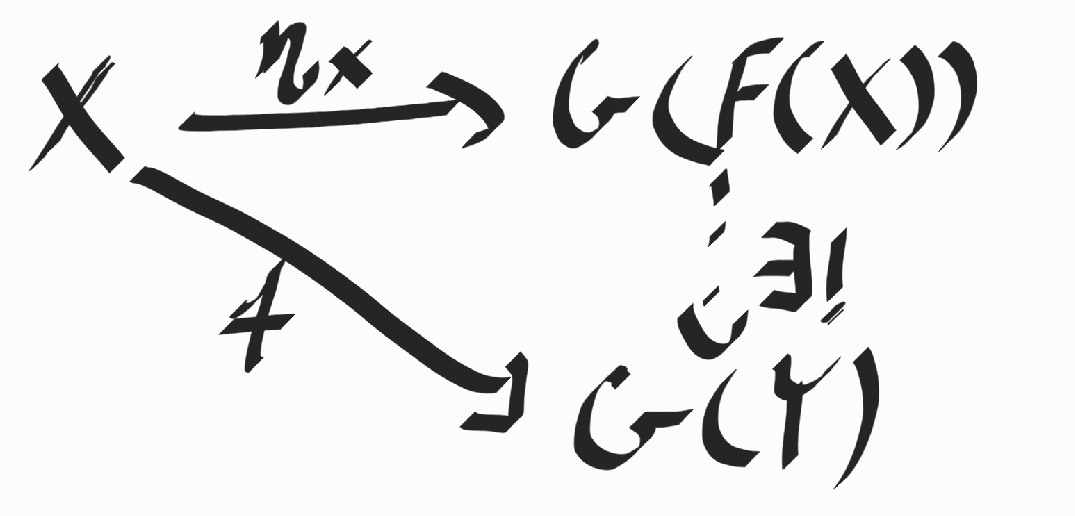
\includegraphics[scale=0.3]{lemma_for_Freid (1).pdf}\end{center}

\\Пусть $F$ у нас есть, возьмём в качестве $\eta_X$ элемент $Hom(X, G(F(X)) \simeq Hom(F(X), F(X))$, соответствующий $id_{F(X)}$.
\\В другую сторону: определим $F(X)$ через лемму Йонеды как объект, такой что $Hom_D(F(X), Y) \simeq Hom_C(X, G(Y))$, $\phi \rightarrow G(\phi) \circ \eta_X$. $f: X \rightarrow X'$, $Hom(F(X), F(X') \simeq Hom(X, G(F(X'))$, определим $F(f)$ как морфизм, соответствующий $\eta_{X'} \circ f$, тогда $G(F(f)) \circ \eta_X = \eta_{X'} \circ f$. Проверим, что $F$ сохраняет композицию:  $X \xrightarrow[]{f} X' \xrightarrow[]{f'} X''$. $F(f' \circ f) = F(f') \circ F(f)$ \Leftrightarrow $G(F(f') \circ F(f)) \circ \eta_X = \eta_{X''} \circ f' circ f$. Левая часть равна $GF(f') \circ GF(f) \circ \eta_X$, правая = $GF(f') \circ \eta_{X'} \circ f = GF(f') \circ GF(f) \circ \eta_X$.

\end{proof}
\end{lemma}
\end{proof}
\end{theorem}


\end{itemize}

\hypertarget{dex}
    \printindex
%staryi_variant
%\hypertarget{uk}{Основные понятия.}
%\begin{multicols}{2}
%    \hyperlink{}{} \ 
%\end{multicols}
%novyi_variant
\end{document}